%picb,picc,picdr,picds,pice,tabb,tabc,tabdr,tabds,tabe
%eqrib,equob

\subsection{Innenwiderstand und Leerlaufspannung der verschiedenen Spannungsquellen}
Trägt man die Messwerte (Tab. \ref{tabb} - \ref{tabds}) der einzelnen Versuche 
auf (Abb. \ref{picb} - \ref{picds}), so lässt sich jeweils eine lineare Regression \cite{linreg}
durchführen und daraus über Gleichung \ref{equk} auf die Leerlaufspannung und den Innenwiderstand
schließen. 
\begin{align}
\text{Monozelle mit Bel}&\text{astungswiderstand (0-50 $\Omega$)} \nonumber \\
U_k&=U_0-I R_i \\
\Leftrightarrow y&=b+a*x \\
\Leftrightarrow U&=1.5927\text{ V}+(-6.5829)\Omega*I \\
-a&=(6.5829\pm 0.1742)\Omega=R_i \label{eqrib}\\
b&=(1.5927\pm 0.0205)\text{ V}=U_0 \label{equob}
\end{align}
\begin{align}
\text{Monozelle mit Belastungswi}&\text{derstand (0-50 $\Omega$) und Gegenspannung (3,575 V)} \nonumber \\
U_k&=U_0+I R_i \\
\Leftrightarrow y&=b+a*x \\
\Leftrightarrow U&=1.6662\text{ V}-6.6078\Omega*I \\
a&=(6.6078\pm 0.2212)\Omega=R_i\\
b&=(1.6662\pm 0.0320)\text{ V}=U_0
\end{align}
\begin{align}
\text{Rechteckspannung mit }&\text{Belastungswiderstand (20-250 $\Omega$)} \nonumber \\
U_k&=U_0-I R_i \\
\Leftrightarrow y&=b+a*x \\
\Leftrightarrow U&=0.5728\text{ V}+(-48.1232)\Omega*I \\
-a&=(48.1232\pm 1.1149)\Omega=R_i\\
b&=(0.5728\pm 0.0050)\text{ V}=U_0
\end{align}
\begin{align}
\text{Sinusspannung mit Belast}&\text{ungswiderstand (0,1-5 k$\Omega$)} \nonumber \\
U_k&=U_0-I R_i \\
\Leftrightarrow y&=b+a*x \\
\Leftrightarrow U&=1.8024\text{ V}+(-535.9086)\Omega*I \\
-a&=(535.9086\pm 4.5713)\Omega=R_i\\
b&=(1.8024\pm 0.0069)\text{ V}=U_0
\end{align}
	\begin{figure}[h]
		\begin{center}
		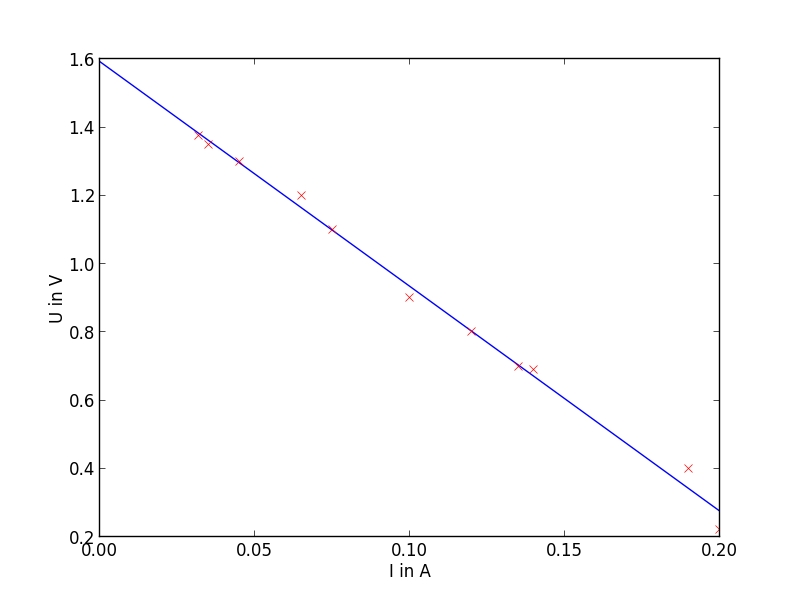
\includegraphics[scale=0.5]{picb.jpg}
		\caption{Monozelle mit Belastungswiderstand (0-50 $\Omega$)}
		\label{picb}
		\end{center}	
	\end{figure} \begin{table}[h]
	\begin{center}
		\begin{tabular}{cc}
			U [V]&I [mA] \\ \hline
			0,220&200\\
			0,400&190\\
			0,690&140\\
			0,700&135\\
			0,800&120\\
			0,900&100\\
			1,100&75\\
			1,200&65\\
			1,300&45\\
			1,350&35\\
			1,375&32
		\end{tabular}
		\caption{Monozelle mit Belastungswiderstand (0-50 $\Omega$)}
		\label{tabb}
	\end{center}
\end{table} 	\begin{figure}[h]
		\begin{center}
		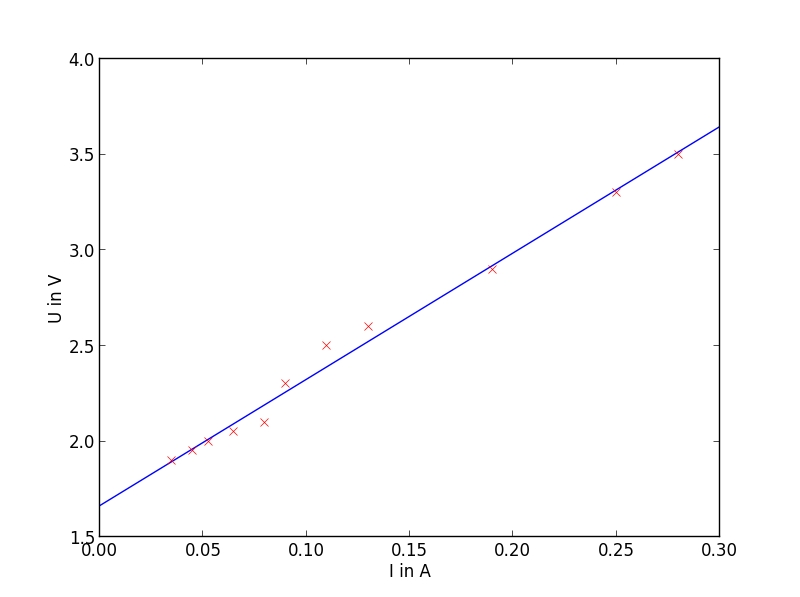
\includegraphics[scale=0.5]{picc.jpg}
		\caption{Monozelle mit Belastungswiderstand (0-50 $\Omega$) und Gegenspannung (3,575 V)}
		\label{picc}
		\end{center}	
	\end{figure}  \begin{table}[h]
	\begin{center}
		\begin{tabular}{cc}
			U [V]&I [mA] \\ \hline
			3,50&280,0\\
			3,30&250,0\\
			2,90&190,0\\
			2,60&130,0\\
			2,50&110,0\\
			2,30&90,0\\
			2,10&80,0\\
			2,05&65,0\\
			2,00&52,5\\
			1,95&45,0\\
			1,90&35,0
		\end{tabular}
		\caption{Monozelle mit Belastungswiderstand (0-50 $\Omega$) und Gegenspannung (3,575 V)}
		\label{tabc}
	\end{center}
\end{table} 	\begin{figure}[h]
		\begin{center}
		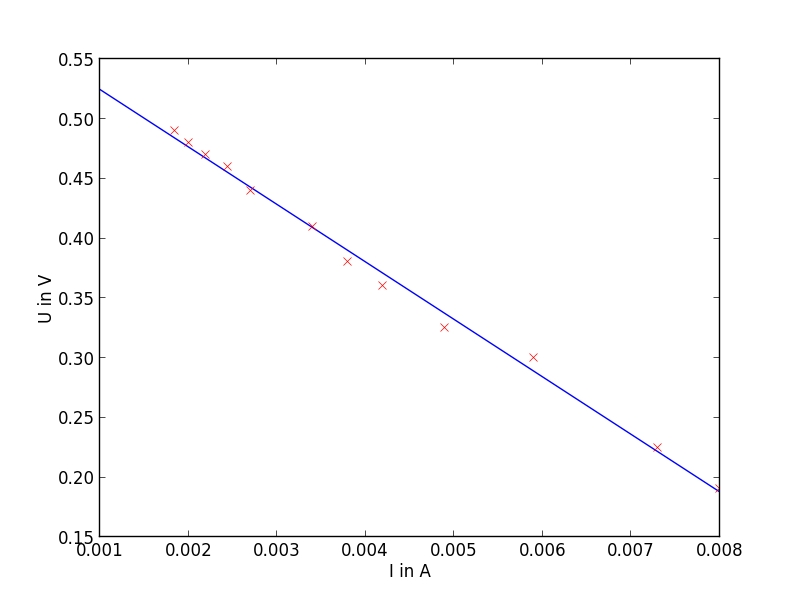
\includegraphics[scale=0.5]{picdr.jpg}
		\caption{Rechteckspannung mit Belastungswiderstand (20-250 $\Omega$)}
		\label{picdr}
		\end{center}	
	\end{figure} \begin{table}[h]
	\begin{center}
		\begin{tabular}{cc}
			U [mV]&I [mA] \\ \hline
			190&8,00\\
			225&7,30\\
			300&5,90\\
			325&4,90\\
			360&4,20\\
			380&3,80\\
			410&3,40\\
			440&2,70\\
			460&2,45\\
			470&2,20\\
			480&2,00\\
			490&1,85
		\end{tabular}
		\caption{Rechteckspannung mit Belastungswiderstand (20-250 $\Omega$)}
		\label{tabdr}
	\end{center}
\end{table} 	\begin{figure}[h]
		\begin{center}
		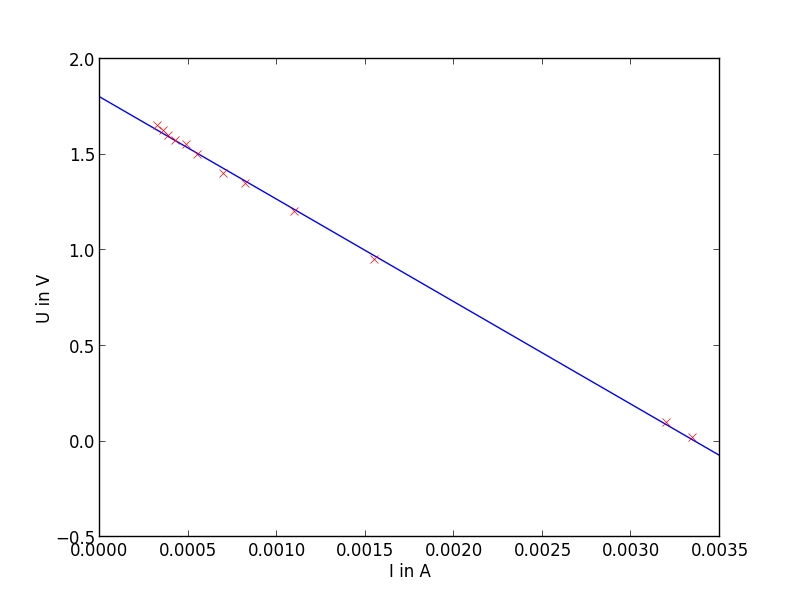
\includegraphics[scale=0.5]{picds.jpg}
		\caption{Sinusspannung mit Belastungswiderstand (0,1-5 k$\Omega$)}
		\label{picds}
		\end{center}	
	\end{figure} \begin{table}[h]
	\begin{center}
		\begin{tabular}{cc}
			U [mV]&I [mA] \\ \hline
			16,5&3,350\\
			95,0&3,200\\
			950,0&1,550\\
			1200,0&1,100\\
			1350,0&0,825\\
			1400,0&0,700\\
			1500,0&0,556\\
			1550,0&0,490\\
			1575,0&0,430\\
			1600,0&0,390\\
			1625,0&0,360\\
			1650,0&0,330
		\end{tabular}
		\caption{Sinusspannung mit Belastungswiderstand (0,1-5 k$\Omega$)}
		\label{tabds}
	\end{center}
\end{table}
\FloatBarrier
\subsection{Direkte Messung der Leerlaufspannung der Monozelle}
Da bei der Messung der Leerlaufspannung $U_0=1,575 \text{ V}$ der Eingangswiderstand $R_V=10\text{M}\Omega$
einen endlichen Wert besaß kommt es mit $R_i=6.5829\Omega$ (Gl. \ref{eqrib}) zu einem Messfehler nach Gleichung \ref{equk}.
\begin{align}
\Delta U_{0}&=\frac{U_{0,mess}}{R_V}*R_i=1,0368*10^{-6}\text{ V}
\end{align}
\subsection{Umgesetzte Leistung des Belastungswiderstandes bei einer Monozelle}
	\begin{figure}[h]
		\begin{center}
		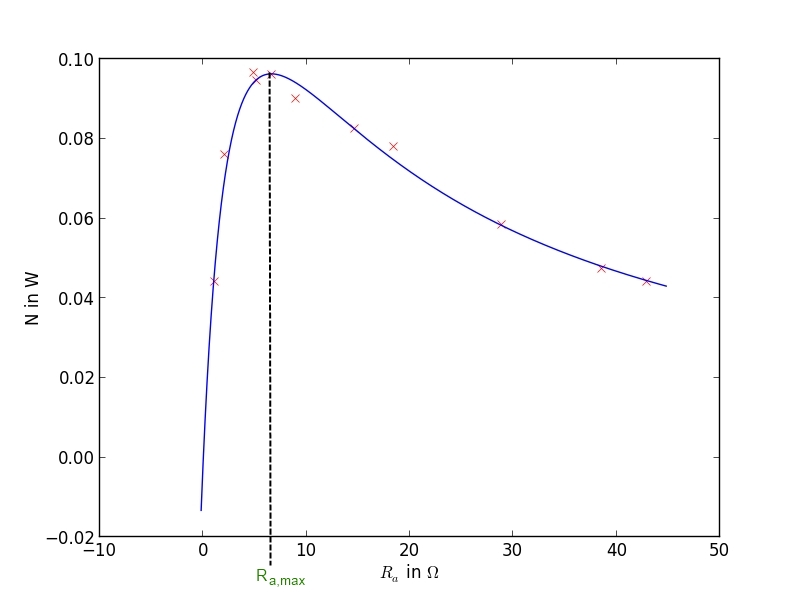
\includegraphics[scale=0.5]{pice.jpg}
		\caption{Umgesetzte Leistung des Belastungswiderstandes (Monozelle)}
		\label{pice}
		\end{center}	
	\end{figure} \begin{table}[h]
	\begin{center}
		\begin{tabular}{cc}
			$R_a$ [$\Omega$]&N [W] \\ \hline
			1,1000&0,0440\\ 
			2,1053&0,0760 \\  
			4,9286&0,0966\\
			5,1852&0,0945 \\
			6,6667&0,0960\\
			9,0000&0,0900\\
			14,6667&0,0825 \\
			18,4615&0,0780 \\
			28,8889&0,0585 \\
			38,5714&0,0473 \\
			42,9688&0,0440
			\end{tabular}
		\caption{Umgesetzte Leistung des Belastungswiderstandes (Monozelle)}
		\label{tabe}
	\end{center}
\end{table}
Aus Tabelle \ref{tabe} lässt sich mit Gleichung \ref{eqn} und \ref{equk} Abbildung \ref{pice} erstellen.
Außerdem ist mit den Werten aus Gleichung \ref{eqrib} und \ref{equob} die Theoriekurve eingezeichnet worden.
\begin{align}
R_a&=\frac{U_k}{I} \\
\Rightarrow N_{Versuch}&=I*U_k \\ 
U_k&=U_0-I R_i \\
\Rightarrow N_{Theorie}&=I (U_0 - I R_i)
\end{align}
\FloatBarrier